\chapter{Implementiertes User Interface}
Nachfolgend wird auf das tatsächlich implementierte User Interface eingegangen.
Dabei werden Unterschiede und Abweichungen zum Entwurf aufgezeigt und das generelle Design wird gezeigt.
Die Bedienung des User Interfaces bleibt dabei größtenteils gleich, somit ist die Bedienungsanleitung des UI Entwurfs nach wie vor maßgebend.
Es wurden hauptsächlich gestalterisch andere, meist bessere Lösungen gefunden.

\section{Unterschiede beim generellen Design}

\begin{wrapfigure}[15]{r}{5.5cm}
  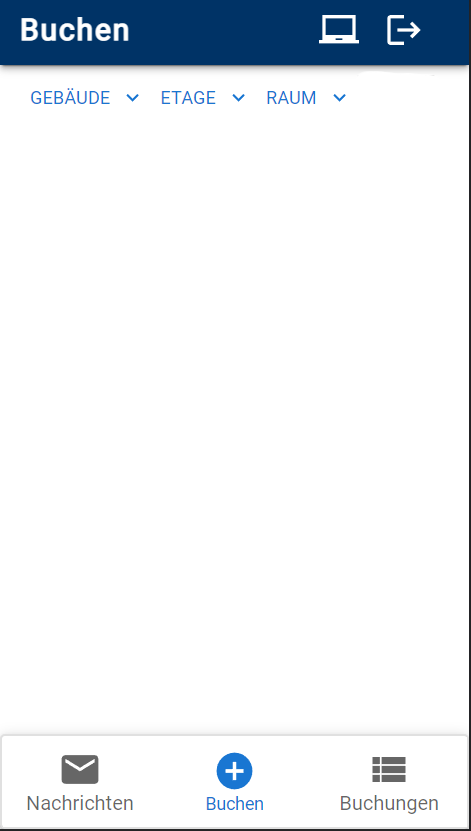
\includegraphics[width=5.5cm]{ImplBuchen.png}
  \caption{User Interface: Buchen}
\end{wrapfigure}

Abbildung 4.1 zeigt das generelle Design der Buchen Seite.
\\
Dabei sind die Dropdownmenüs aus der oberen Appleiste nach unten gerutscht und wurden visuell ruhiger und simpler gestaltet.
\\
In der oberen Appleiste rechts, wurden noch zwei Buttons hinzugefügt. Der rechte Button zum Ausloggen aus dem System und der linke Button um zu dem Raumeditor zu gelangen, falls ein Admin diesen betätigt
\\\\
In der unteren Auswahlleiste wird die ausgewählte Seite, spricht das Symbol nun nicht wie im Entwurf in schwarz und mit Balken unterhalb hervorgehoben, sondern in einfachen hellblau.

\newpage

\begin{wrapfigure}[14]{r}{5.5cm}
  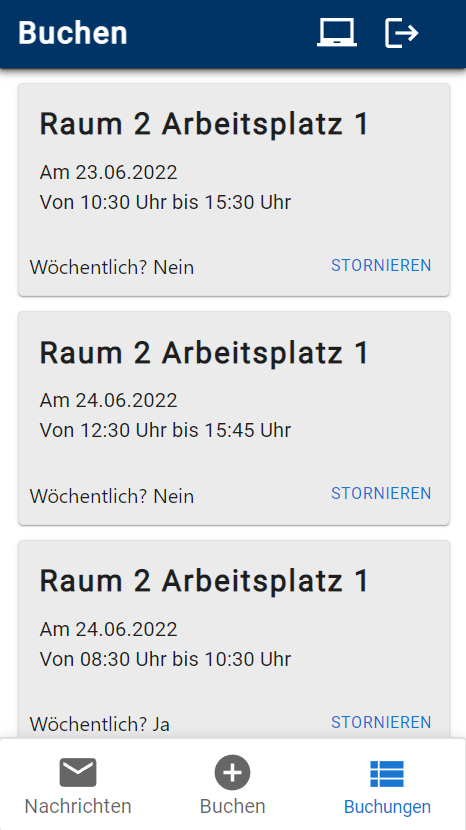
\includegraphics[width=5.5cm]{ImplChronik.png}
  \caption{UI: Buchungen Übersicht}
\end{wrapfigure}

In der Chronik der selbst getätigten Buchungen hat sich nicht viel verändert, bis auf das Design.
\\
Die Einträge Kacheln haben einen weniger markanten Rand und es wurde der Hinweis hinzugefügt, ob es sich bei der Buchung um eine wöchentliche Buchung handelt.
Wöchentliche Buchungen sind fortlaufende Abonnement Buchungen, die jede Woche sich am selben Tag wiederholen und dabei denselben Zeitraum und Arbeitsplatz haben.
\paragraph{}
Bei der persönlichen Nachrichtenübersicht hat sich ebenfalls nur das Kacheldesign geändert und ist damit angepasst an die Kacheln der Buchungschronik.
Bei den Direktchats blieb alles beim Alten.
\vspace{29mm}
\begin{figure}[!h]
  \centering
  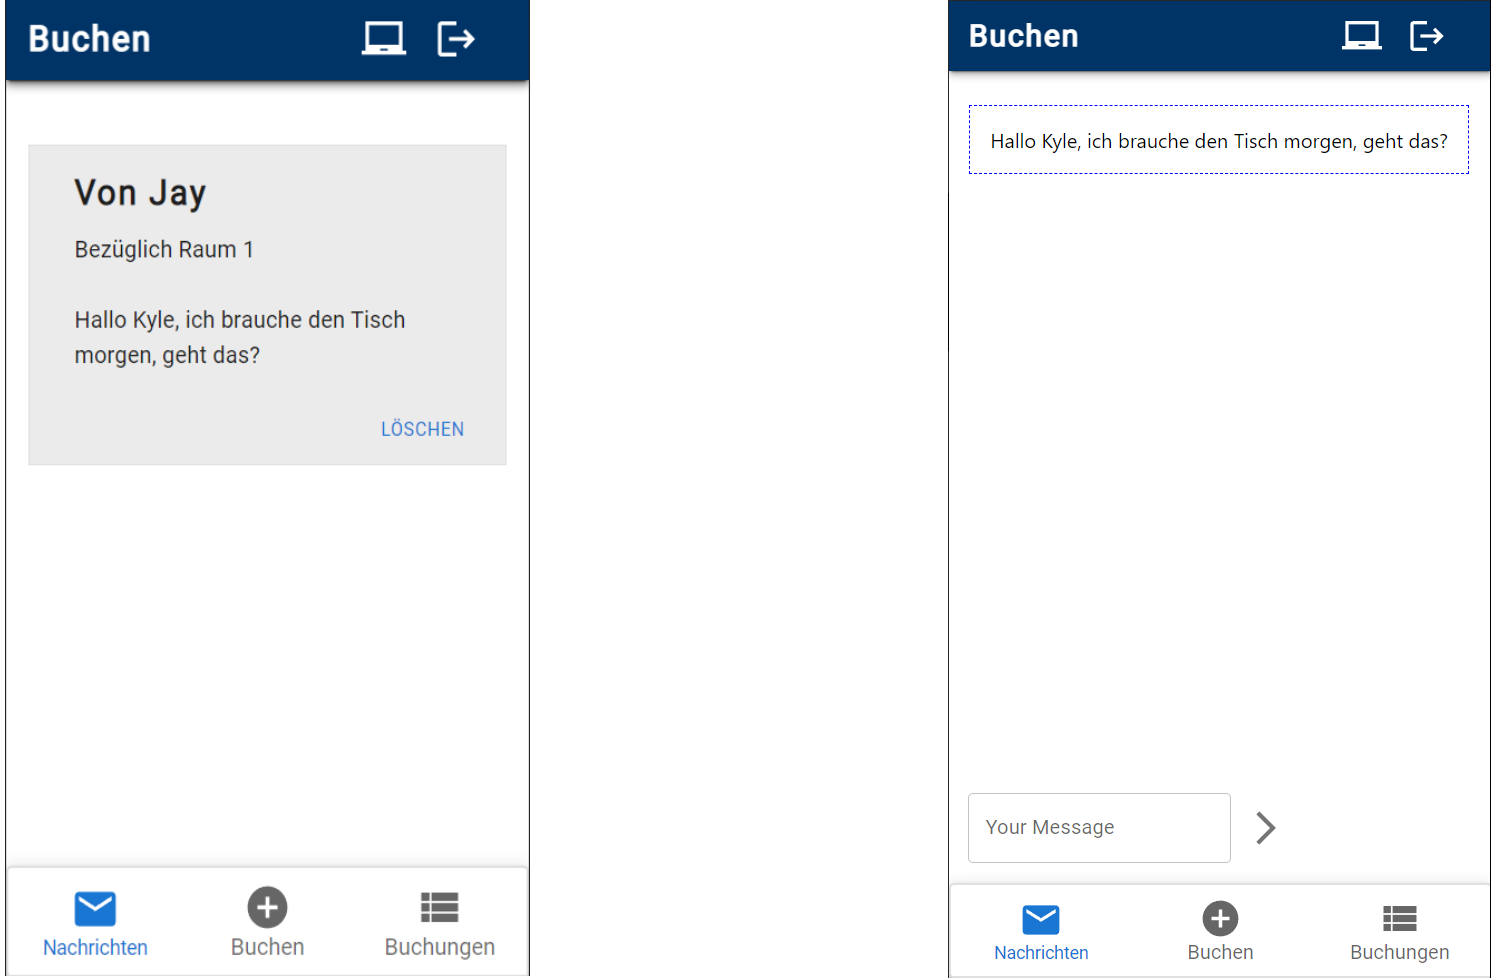
\includegraphics[width=1\textwidth]{ImplNachrichtenGes.png}
  \caption{User Interface: Nachrichten}
  \label{fig:UI_Messages}
\end{figure}

\newpage

\section{Unterschiede des Zeitauswahl Pop-Ups}

\begin{figure}[!h]
  \centering
  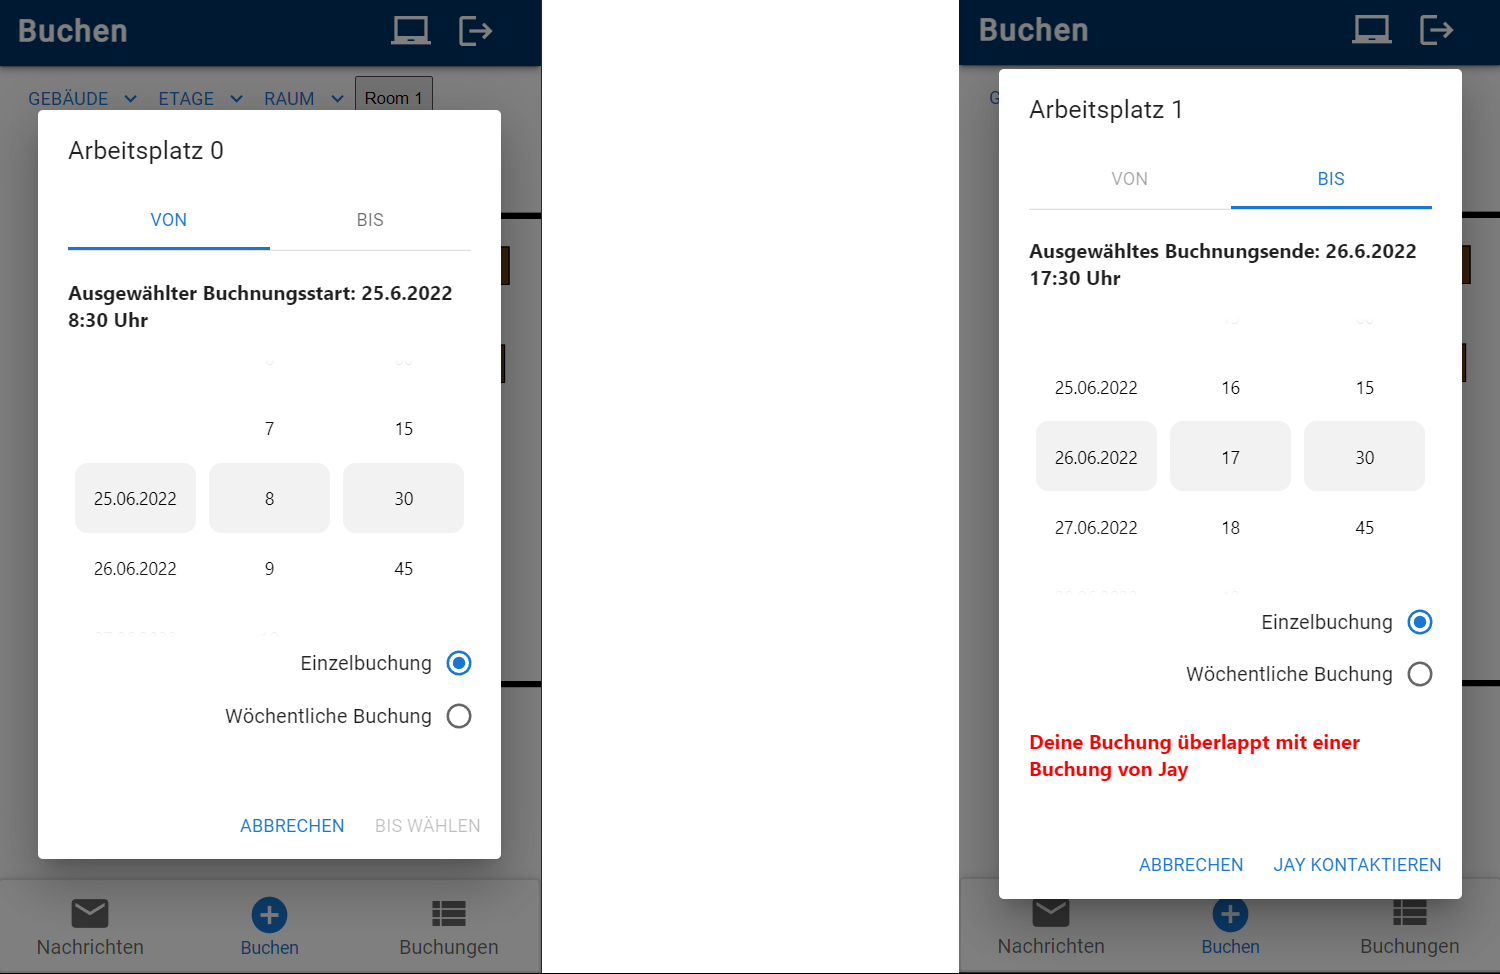
\includegraphics[width=1\textwidth]{ImplPopup12.png}
  \caption{User Interface: Zeitauswahl Pop-Up}
  \label{fig:UI_timePopUp}
\end{figure}

Der Aufbau des Zeitauswahl Pop-Ups ist im Grunde noch gleich, es wurden nur ein paar Regelungen festgelegt beim Eingeben des Zeitraumes und der Überprüfung der Buchung auf Kollisionen mit anderen Buchungen.
\paragraph{}
Zunächst wurde unterhalb der Tabs, Text hinzugefügt, um verständlicher zu machen, was gerade für eine Zeit eingegeben wird.
Dort wird angezeigt, ob gerade der Buchungsstart eingegeben wird oder das Ende, sowie die aktuell gewählte Zeit.
\\\\
Neu mit dazu kamen auch Optionen, eine Dauerbuchung oder Einzelbuchung zu tätigen mit den Radiobuttons Einzel- oder Wöchentliche Buchung.
\paragraph{}
Es wurde nun auch beschränkt, dass nach dem Eingeben einer Endzeit, mit Klicken auf den BIS Tab, die Startzeit nicht mehr verändert werden kann.
Dies sollte für mehr Linearität und Klarheit beim Buchungsprozess sorgen.

\paragraph{}
Die Kollisionserkennung von Buchungszeiträumen wurde nun wesentlich anders gelöst, wie im Entwurf.
\\
Nun wird nach Überschneidungen von verschiedenen Buchungen nämlich erst mit Absenden der Buchung gecheckt, nämlich mit dem Klicken auf den Buchen Button.
Die im Entwurf gewählte Darstellung mit Färben der Daten und Zeiten, bot letztlich wenig Übersicht über andere Buchungen.
Dies kam zustande, weil die Daten oberhalb und unterhalb der ausgewählten mittleren Zeitlinie nicht Anschluss- oder vorangegangene Zeitschlitze sind,
sondern immer um einen Tag und eine Stunde vom nächsten Zeitschlitz entfernt sind. 
Somit könnte nur die mittlere Zeile eingefärbt werden und deshalb wurde dieses Feature eingestellt, weil es zu mehr Verwirrung als Nutzen führen könnte.
\paragraph{}
Nun wird eben mit Klicken des Buchen Buttons ein Hinweistext angezeigt, welcher darauf hindeutet, dass persönlich eine andere Buchung in dem Buchungszeitraum vorliegt oder dass ein Kollege dort eine Buchung hat.
Im Falle der eigenen Buchung bleibt nur die Option Abbrechen, während bei einer Buchung von einem Kollegen man diesen auch anschreiben könnte.

\newpage
\section{Räume und Raumeditor}

\begin{figure}[!h]
  \centering
  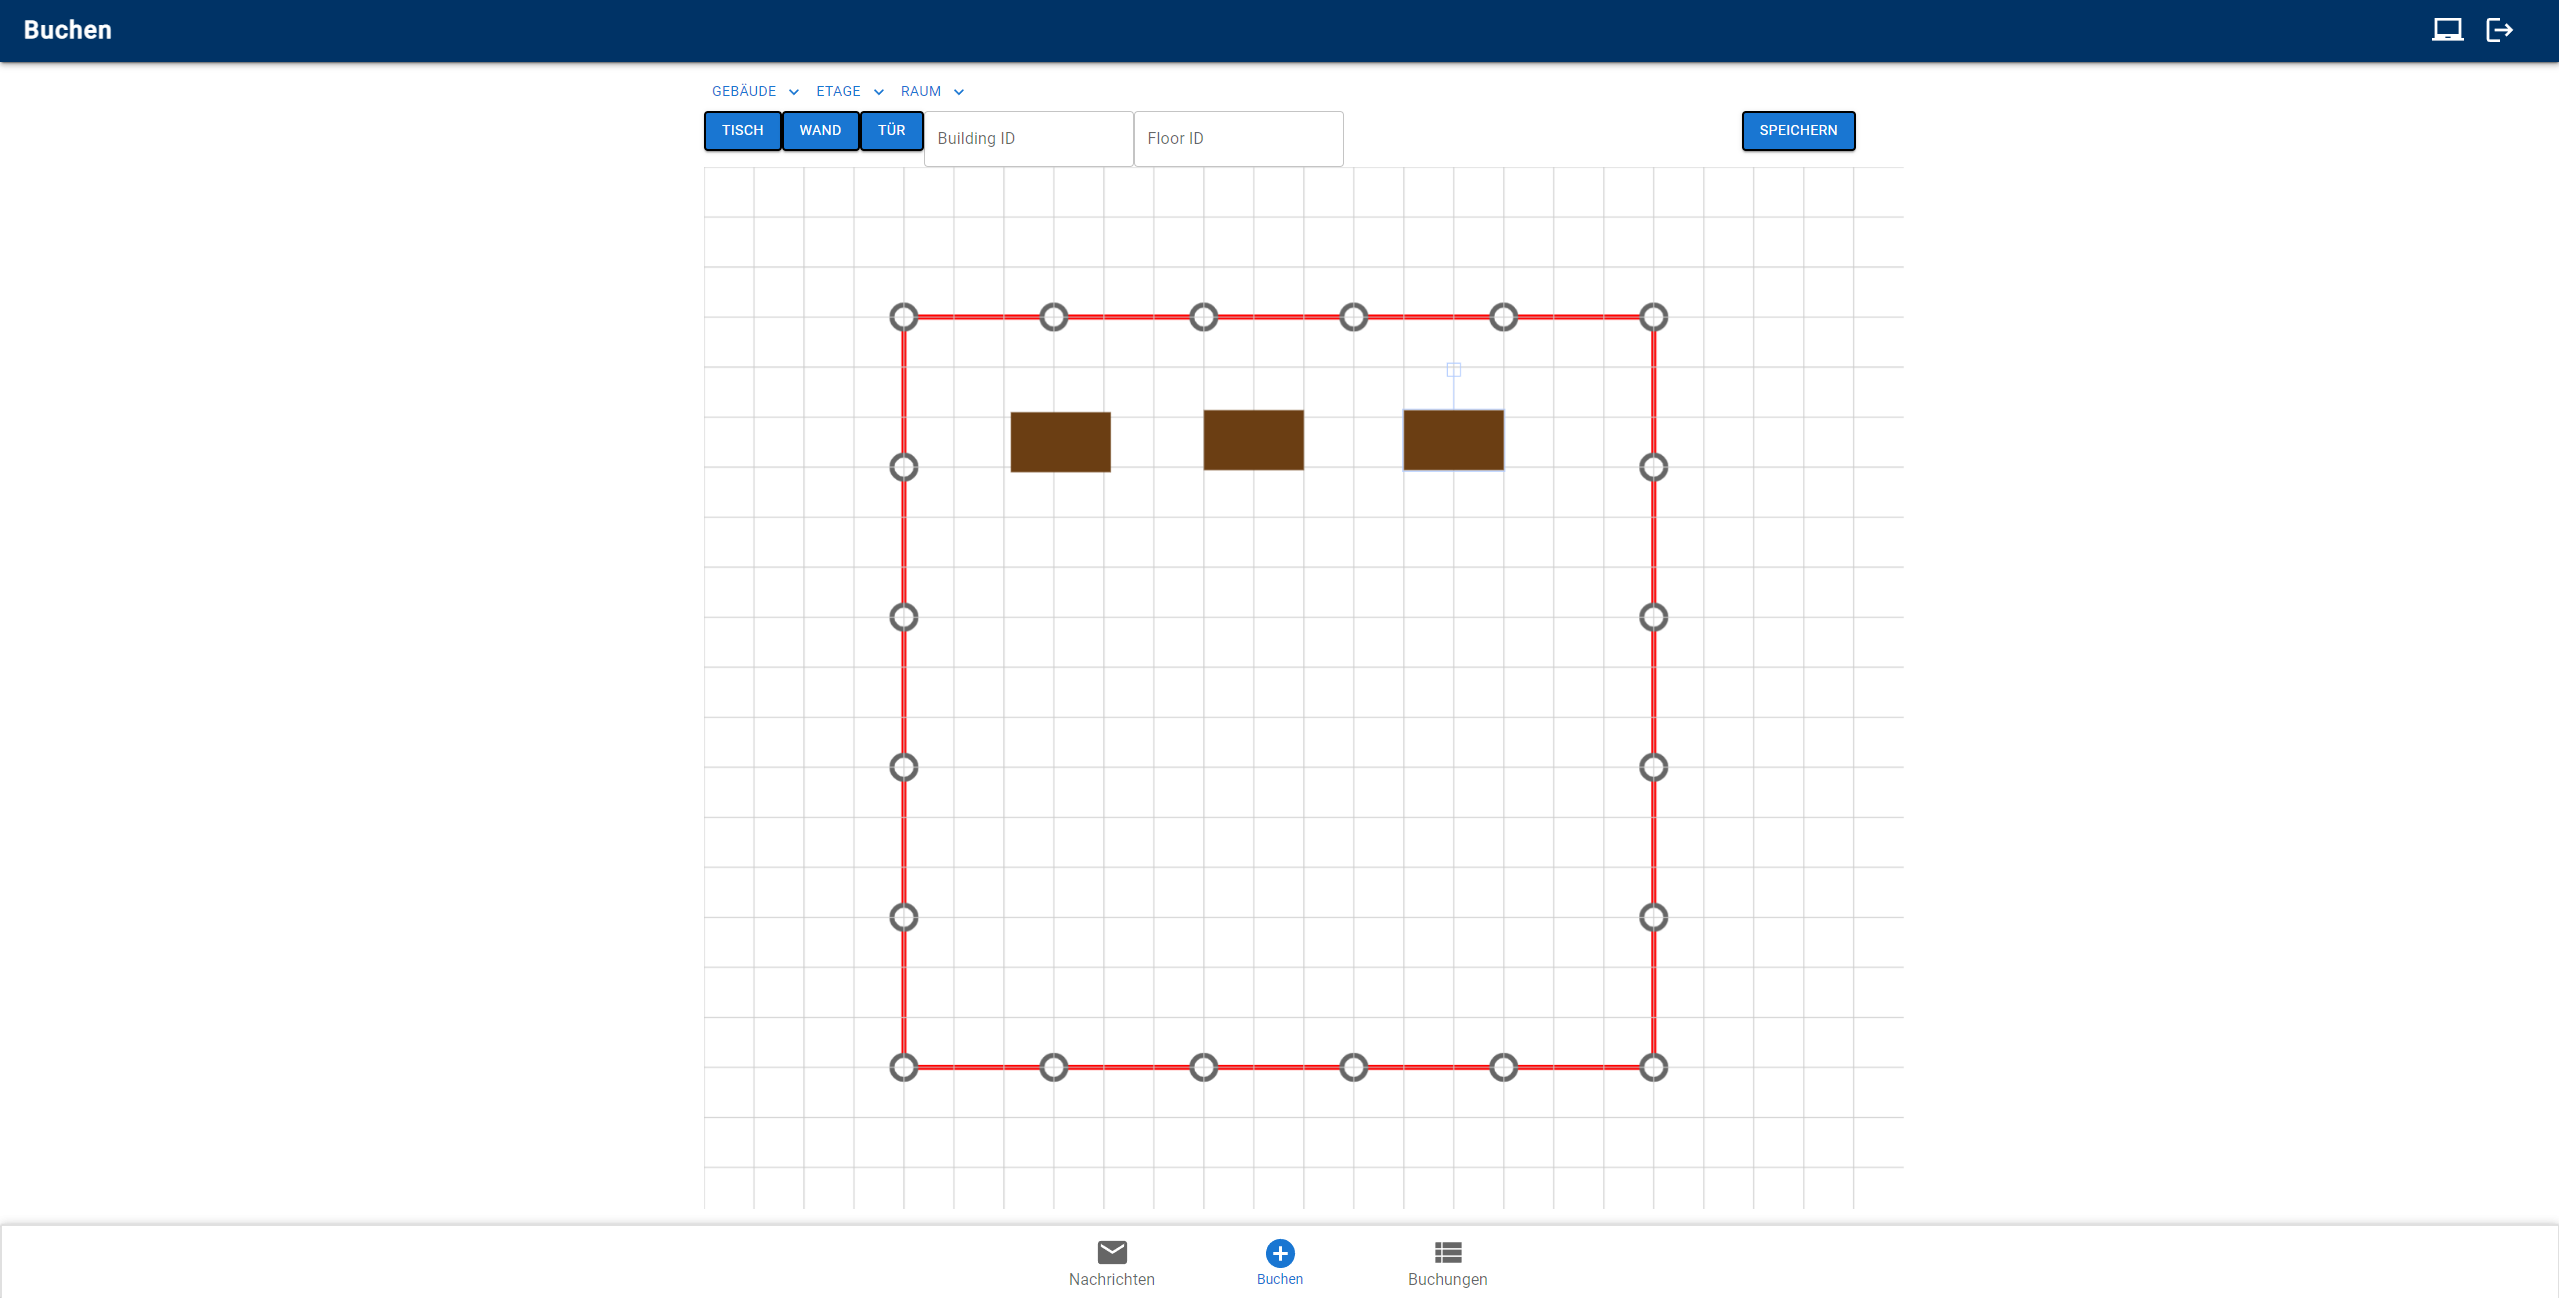
\includegraphics[width=1\textwidth]{ImplEditor.png}
  \caption{User Interface: Raum Editor}
  \label{fig:UI_Editor}
\end{figure}

Abbildung 4.5 zeigt den Stand des Raumeditors. 
\\
Der Raumeditor besitzt in der aktuellen Implementierung eine feste Anzahl an Raum-Eckpunkten, die sich verschieben lassen.
Mit diesen Raumpunkten sind schon einige Räume nachbildbar und die feste Anzahl erleichterte uns die Implementierung des Editors.
\\
Tische sind nun mit einem Doppelklick auf der Bearbeitungfläche erzeugbar. Diese sind verschiebbar und rotierbar.
Diese Erstellung der Tische ermöglich einen schnelleren Workflow, da nicht, wie im Entwurf, immer zuerst die Schaltfläche für einen Tisch gedrückt werden muss.
Der Speicher Button ist nun oberhalb des Zeichenfeldes. 
\\
Ebenfalls ist es nun möglich zwischen dem Raumeditor und dem restlichen Deskplanner hin und her zu wechseln, durch die Einblendung der oberen Appleiste und unteren Navigationsleiste.
\\\\
Weitere Features des Raumeditors, die im Entwurf vorhanden sind und in der Implementierung nicht, werden im Ausblick der Dokumentation behandelt.


